\documentclass{article}%
\usepackage[T1]{fontenc}%
\usepackage[utf8]{inputenc}%
\usepackage{lmodern}%
\usepackage{textcomp}%
\usepackage{lastpage}%
\usepackage[head=40pt,margin=0.5in,bottom=0.6in]{geometry}%
\usepackage{graphicx}%
%
\title{\textbf{Siete cadáveres de mineros fueron llevados a un fuerte militar}}%
\author{ZULVYN DÍAZ | zndiaz@el.nacional.com}%
\date{18/10/2018}%
%
\begin{document}%
\normalsize%
\maketitle%
\textbf{URL: }%
http://www.el{-}nacional.com/noticias/sucesos/siete{-}cadaveres{-}mineros{-}fueron{-}llevados{-}fuerte{-}militar\_256224\newline%
%
\textbf{Periodico: }%
EN, %
ID: %
256224, %
Seccion: %
Sucesos\newline%
%
\textbf{Palabras Claves: }%
Sucesos, Bolívar\newline%
%
\textbf{Derecho: }%
3.2, %
Otros Derechos: %
1.10, %
Sub Derechos: %
3.2.1, 1.10.1.1\newline%
%
\textbf{EP: }%
SI\newline%
\newline%
%
\textbf{\textit{Por cuarto día consecutivo residentes de la zona protestaron y mantienen cerrada la carretera Troncal 10}}%
\newline%
\newline%
%
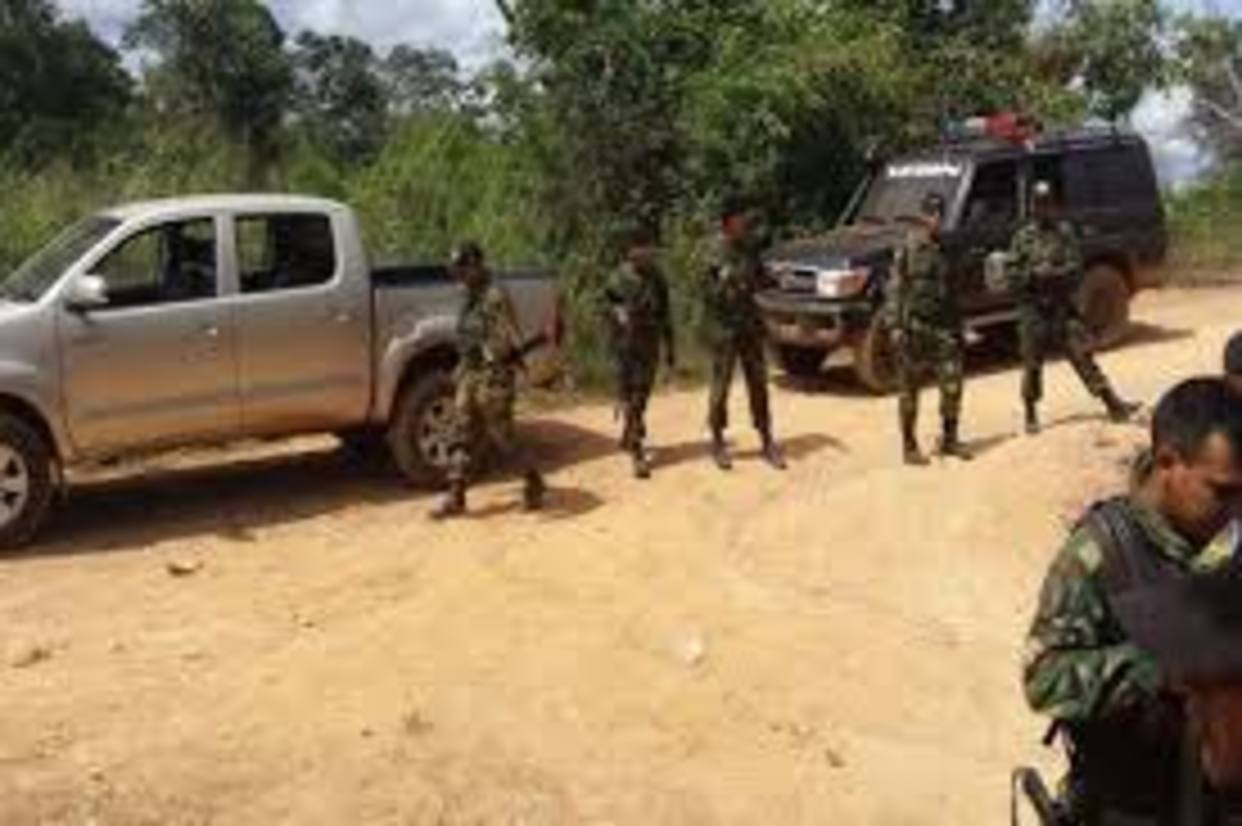
\includegraphics[width=300px]{243.jpg}%
\newline%
%
Los cuerpos de cuatro hombres y tres mujeres, en avanzado estado de descomposición y con heridas de arma de fuego, fueron trasladados por comisiones policiales y del Ejército al Fuerte Militar Tarabay, a la espera de ser identificadas por un grupo de especialistas enviados desde Caracas y Ciudad Guayana.%
\newline%
%
El Ministerio Público designó ayer a la Fiscalía 5a~de Tumeremo para que inicie la investigación del caso, cinco días después de haber ocurrido la matanza de mineros. Este hecho es el cuarto que ocurre en la zona desde el año 2016, cuando el gobierno creó el Arco Minero del Orinoco e inició las exploraciones del terreno en septiembre de ese año.%
\newline%
%
Se conoció que una comisión del Servicio Bolivariano de Inteligencia Nacional, la Guardia Nacional Bolivariana, el Ejército, la Dirección General de Contrainteligencia Militar y el Cicpc se trasladó ayer para comenzar las investigaciones sobre lo ocurrido.%
\newline%
%
Las víctimas fueron halladas por comisiones mixtas integradas por funcionarios del Cuerpo de Investigaciones Científicas, Penales y Criminalísticas de Tumeremo y militares del Ejército, en el sector La Y, en la vía que conduce a la mina El Candado~el martes en la noche, aseguró el diputado Américo De Grazia.%
\newline%
%
Se presume que las 7 víctimas forman parte del grupo de 16 personas trabajadoras de la mina El Candado, que fueron reportadas como desaparecidas por sus familiares el domingo, cuando en el sector se presentó el supuesto enfrentamiento entre miembros de la banda del Coporo y el Ejército de Liberación Nacional, de Colombia, aseguró De Grazia.%
\newline%
%
El martes en la noche, al conocerse el hallazgo, los familiares de los desaparecidos, en compañía de trabajadores de la mina y otros residentes de la localidad, se trasladaron hasta el Fuerte Militar para obtener información, según la clasificación oficial de las víctimas; sin embargo, los funcionarios se mantuvieron herméticos ante la demanda, dijo el parlamentario.%
\newline%
%
A pesar de que los habitantes de la zona aseguraron que los trabajadores del oro no están desaparecidos sino muertos en el tiroteo ocurrido el domingo, ninguna autoridad ha fijado posición. Familiares y habitantes del sector mantienen por cuarto día consecutivo el cierre de la Troncal~10, a~la altura del terminal de pasajeros para exigir celeridad en la búsqueda del resto de las víctimas, la entrega de los cuerpos y una respuesta de las autoridades acerca de lo ocurrido.%
\newline%
%
La localidad permanece en toque de queda impuesto por la banda criminal del Coporo, a la espera de la entrega de los cuerpos. Desde el lunes, la situación mantiene cerrados los comercios, las escuelas y los liceos, sin que las autoridades hayan intervenido a pesar de ser una zona militarizada.%
\newline%
%
\end{document}